%!TEX root = ../thesis.tex
% ******************************* Thesis Appendix A ****************************


\ifpdf
\graphicspath{{Appendix1/Figs/Raster/}{Appendix1/Figs/PDF/}{Appendix1/Figs/}}
\else
\graphicspath{{Appendix1/Figs/Vector/}{Appendix1/Figs/}}
\fi



\chapter{Data quality and errors} 

%\section{Experimental procedure} 
%The Yellow Fluorescent Protein (YFP) marker for the plasma membrane was
%amplified using PCR with primers attb1-mYfwd
%(5'-AGAAAGCTGGGTTTACTTGTACAGCTCGTCCATGCCGAGAGTG) and attb2-YFPrev
%(5'-AGAAAGCTGGGTTTACTTGTACAGCTCGTCCATGCCGAGAGTG), with the forward primer
%sequence containing a motif known to acetylate in plant cells~CITEHERE. 50
%$\mu$L solution was amplified in 96 $^\circ$C for 1 minute, followed by 25
%cycles of 96 $^\circ$C for 30 seconds, and a final elongation for 30 seconds. 5
%$\mu$L of the result was then used in a second reaction consisting of
%40~$\mu$L solution in total, with primers B1 adapt (5'-GGGGACAAGTTTGTACAAAAAAGCAGGCT)
%and B2 adapt (5'-GGGGACCACTTTGTACAAGAAAGCTGGGT) included. Similar to the first
%solution, the second mixture was amplified by PCR in 95 $^\circ$C for 2 minutes,
%followed by 94 $^\circ$C for 30 seconds, 48 $^\circ$C for 30 seconds, and 72
%$^\circ$C for 1 minute, 20 cycles of 94 $^\circ$C for 30 seconds,
%55 $^\circ$C for 30 seconds, and 72 $^\circ$C for 1 minute. Finally, elongation
%took place under 72 $^\circ$C for 1 minute.
%Membrane \\
%Nuclei \\
%Unnused data (PIN) \\


\section{Tracking errors}
\label{sec:data_errors}
\begin{figure}[p]
    \centering
        \centering
        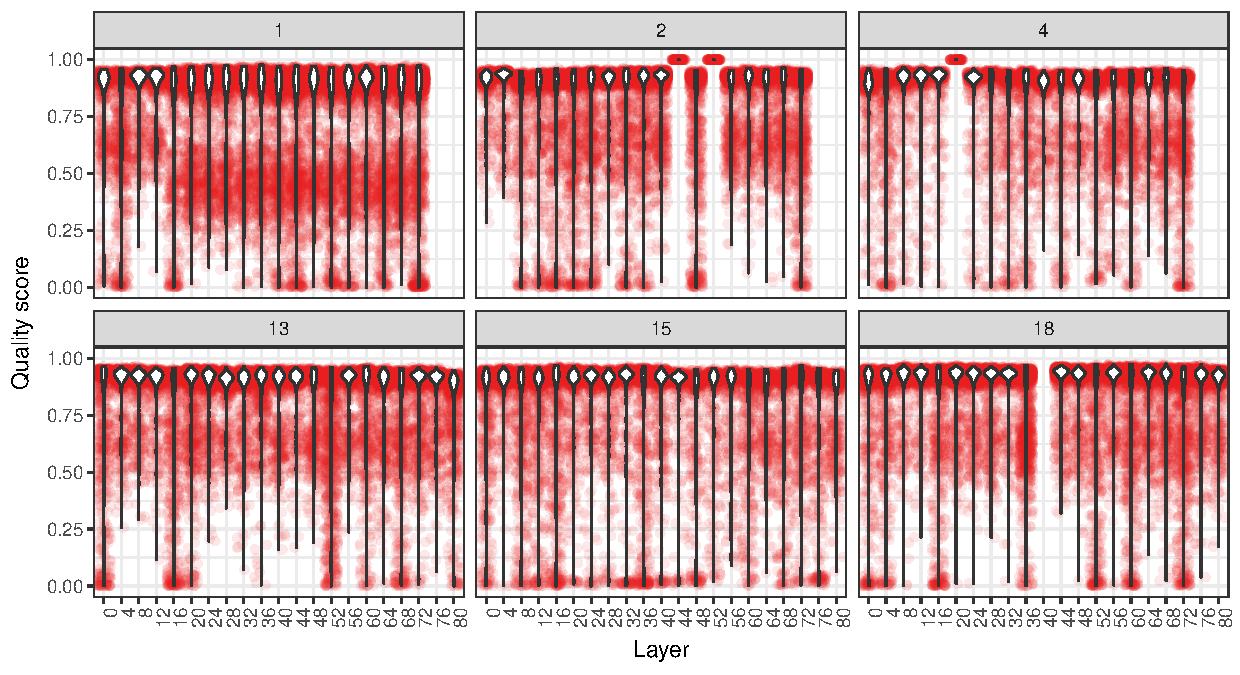
\includegraphics[width=.95\textwidth]{tracking_quality_plant.pdf}
        \centering
        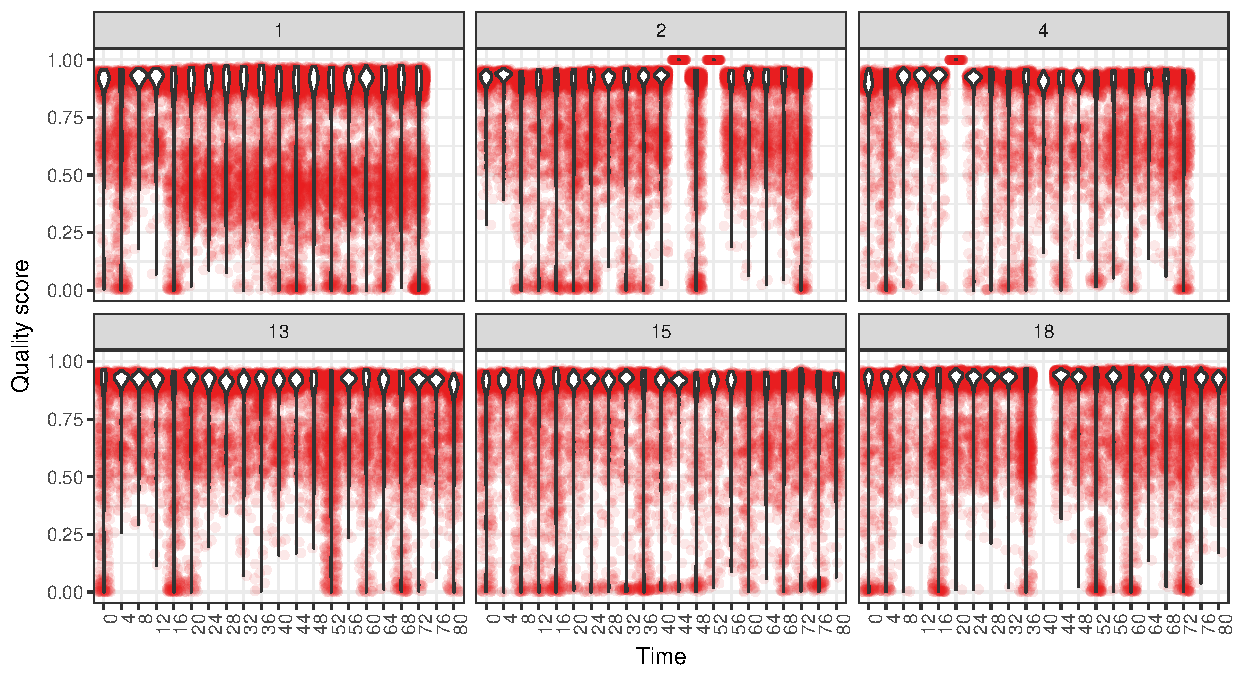
\includegraphics[width=.95\textwidth]{tracking_quality_time.pdf} % second figure itself
        \caption[Tracking quality]{Quality distributions per plant and timepoint for all plants.
        Some timepoints have distributions scoring in the $\sim$1 regime, which
        corresponds to situations where the automatic tracking failed. These
        timepoints have been manually tracked for cells in the L1 within 30
        $\mu$m of the topmost CLV3 expressing cell.}
\end{figure}

\section{Segmentation errors}
\label{sec:data_errors_segmentation}
Discussion of quality decay with increasing d2t.


%\subsubsection{Tracking errors}
%\label{sec:data_errors_tracking}
%Manual tracking in some timepoints...
%\section{Layer Quality Assessment}



